% \section{Atividades}
%
% Neste módulo, foram realizadas atividades práticas voltadas à análise e
% configuração de parâmetros de rede em ambientes Linux e Windows Server 2022,
% com foco em mecanismos de resolução de endereços, endereçamento lógico
% adicional, manipulação de identidade de interface e controle de tráfego.
%
% As tarefas em ambiente Kali Linux contemplaram a observação dinâmica da tabela
% ARP, a criação de aliases de interface de rede, a clonagem de endereço MAC e a
% aplicação de políticas de Qualidade de Serviço (QoS) por meio do utilitário
% \textit{tc}. Em ambiente Windows Server 2022, foi realizada a configuração de
% política de QoS baseada em diretivas locais para limitação de taxa de upload.
%
% Cada atividade apresenta abaixo o respectivo print solicitado, acompanhado de
% descrição explicativa conforme exigido nas orientações do módulo.
%
% \newpage
%
\question[Atividade 11.1]{Explorando a tabela ARP no Kali Linux}

\begin{figure}[H]
\centering
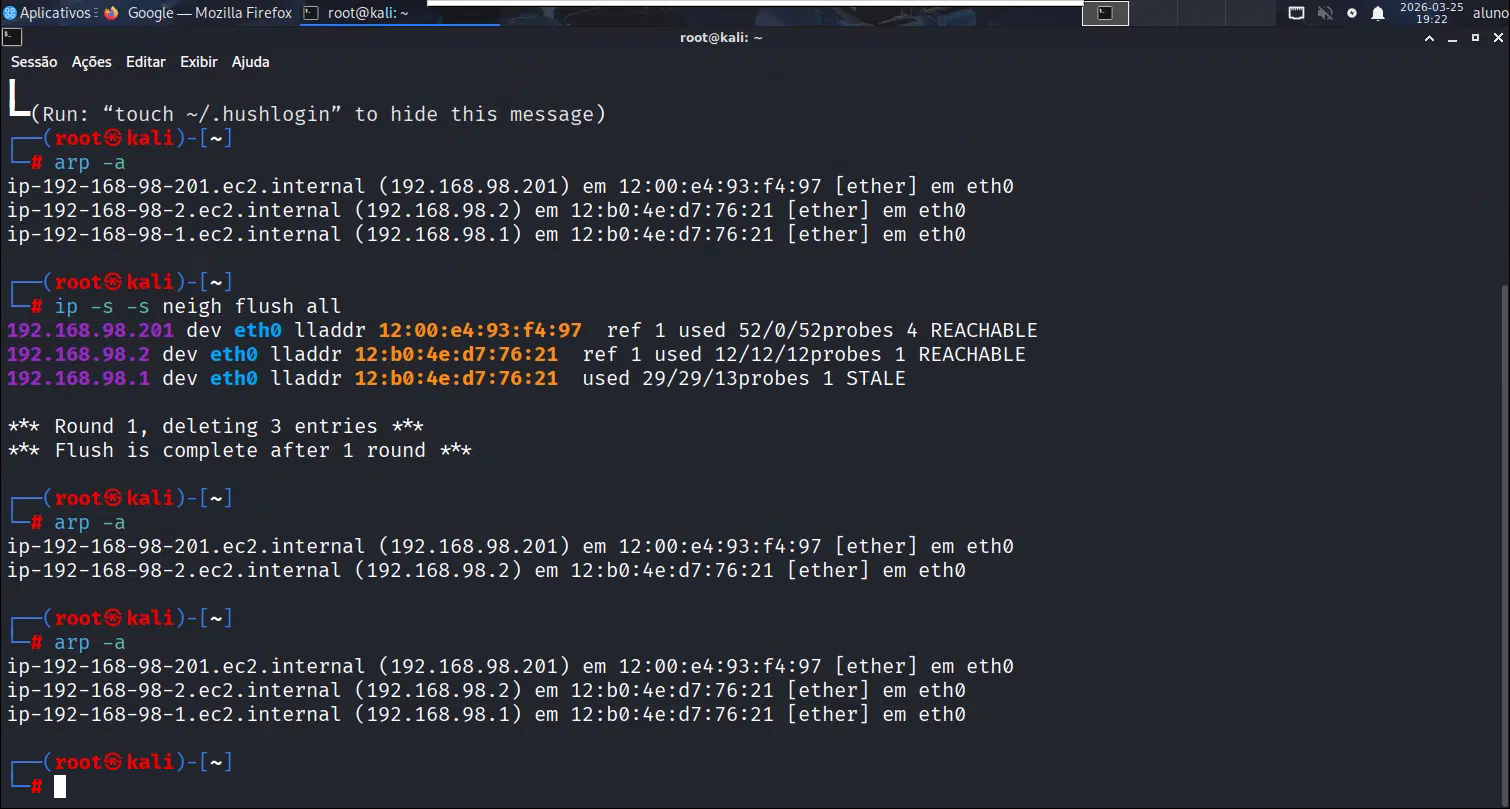
\includegraphics[width=0.99\textwidth]{./fig/fig11.1.png}
\caption{Tabela ARP no Kali Linux após acesso externo, mostrando novamente a entrada do gateway da rede}
\label{fig:fig11.1}
\end{figure}

\newpage

\question[Atividade 11.2]{Implementando Alias de Interface de Rede no Kali Linux}

\begin{figure}[H]
\centering
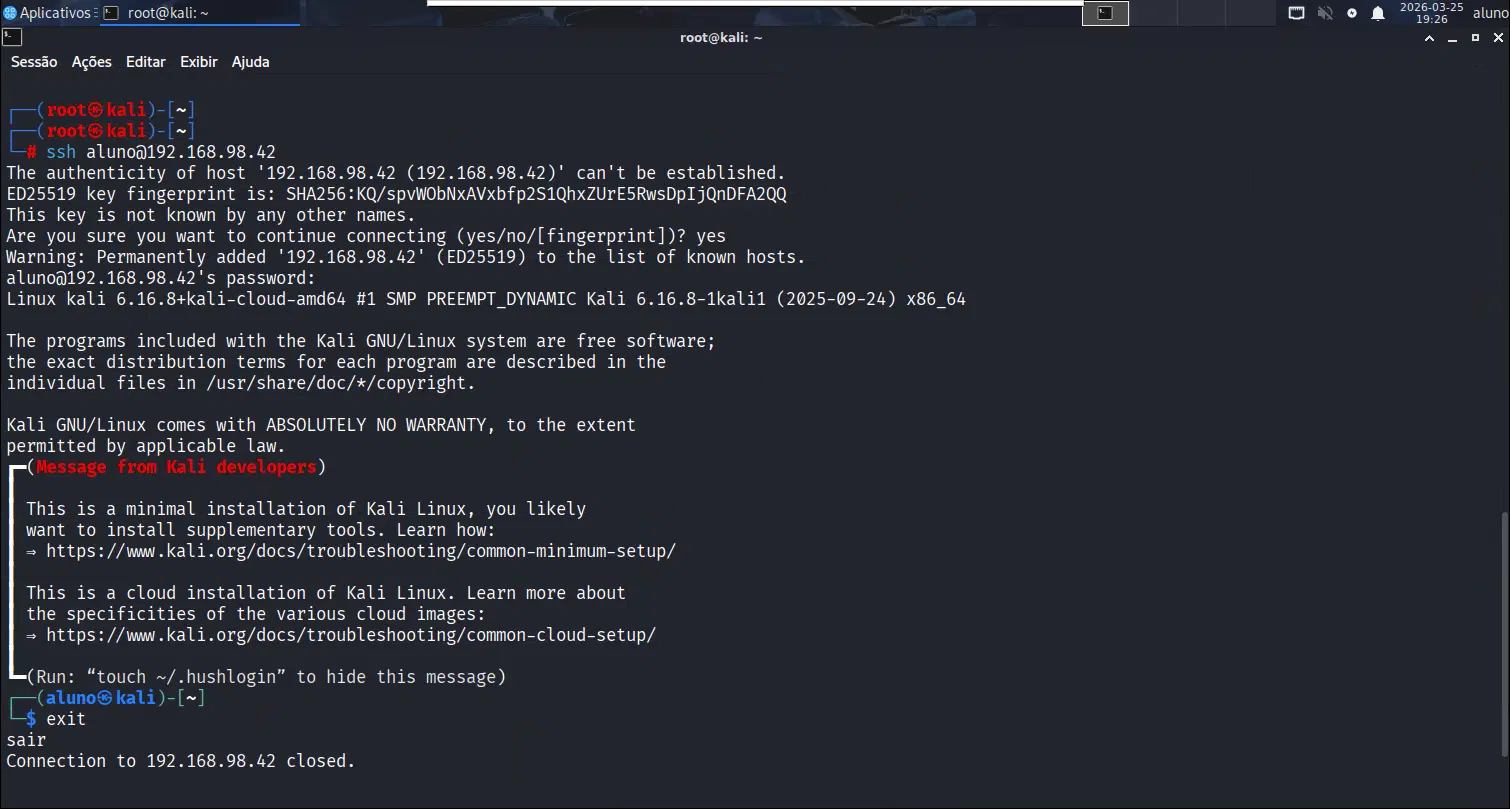
\includegraphics[width=0.99\textwidth]{./fig/fig11.2.png}
\caption{Conexão SSH estabelecida utilizando o alias de interface configurado em 192.168.98.42}
\label{fig:fig11.2}
\end{figure}

\newpage

\question[Atividade 11.3]{Implementando MAC Cloning no Kali Linux}

\begin{figure}[H]
\centering
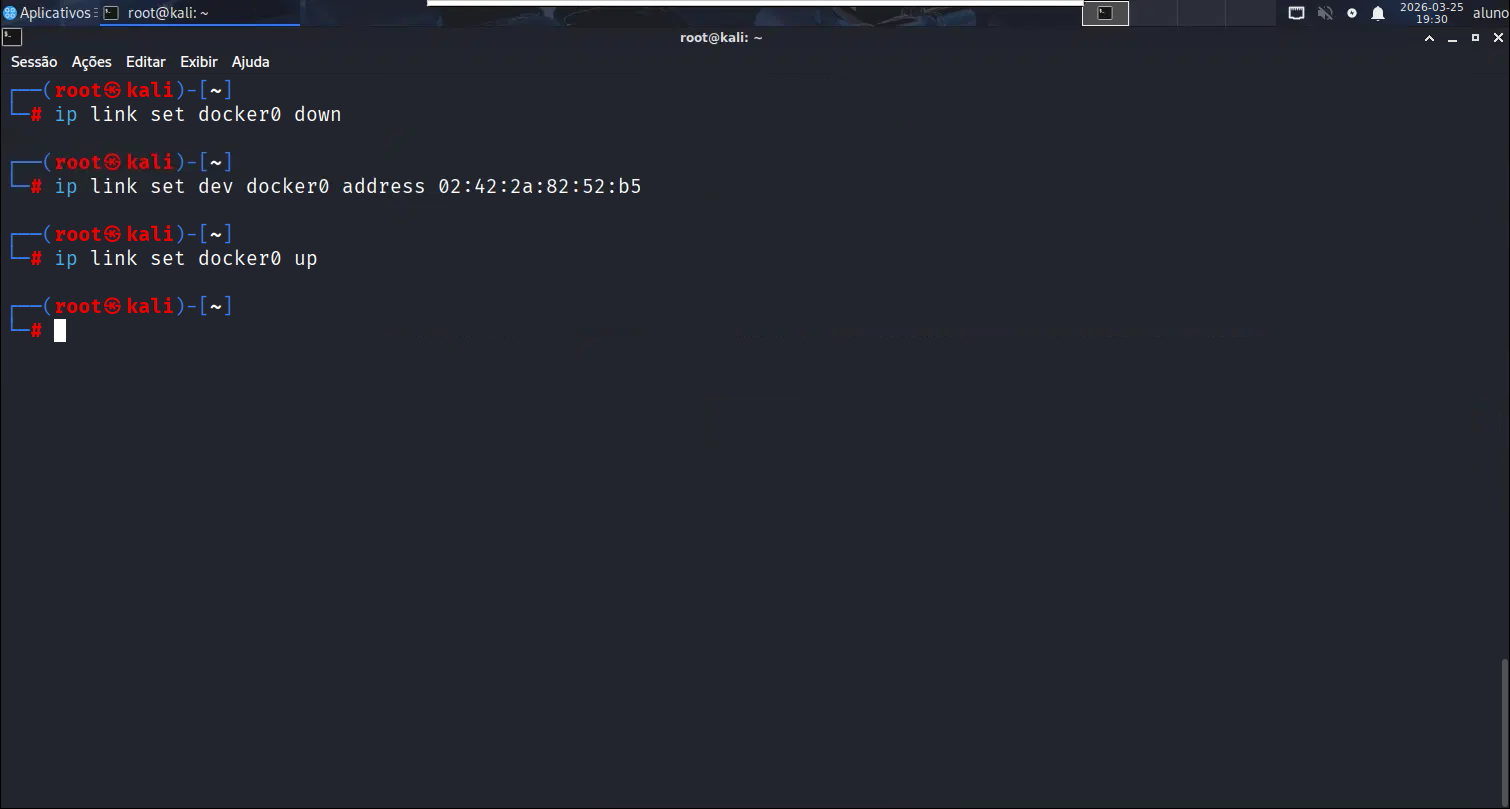
\includegraphics[width=0.99\textwidth]{./fig/fig11.3.png}
\caption{Reconfiguração da interface docker0 com retorno ao endereço MAC original}
\label{fig:fig11.3}
\end{figure}

\newpage

\question[Atividade 11.4]{Configurando QoS no Kali Linux}

\begin{figure}[H]
\centering
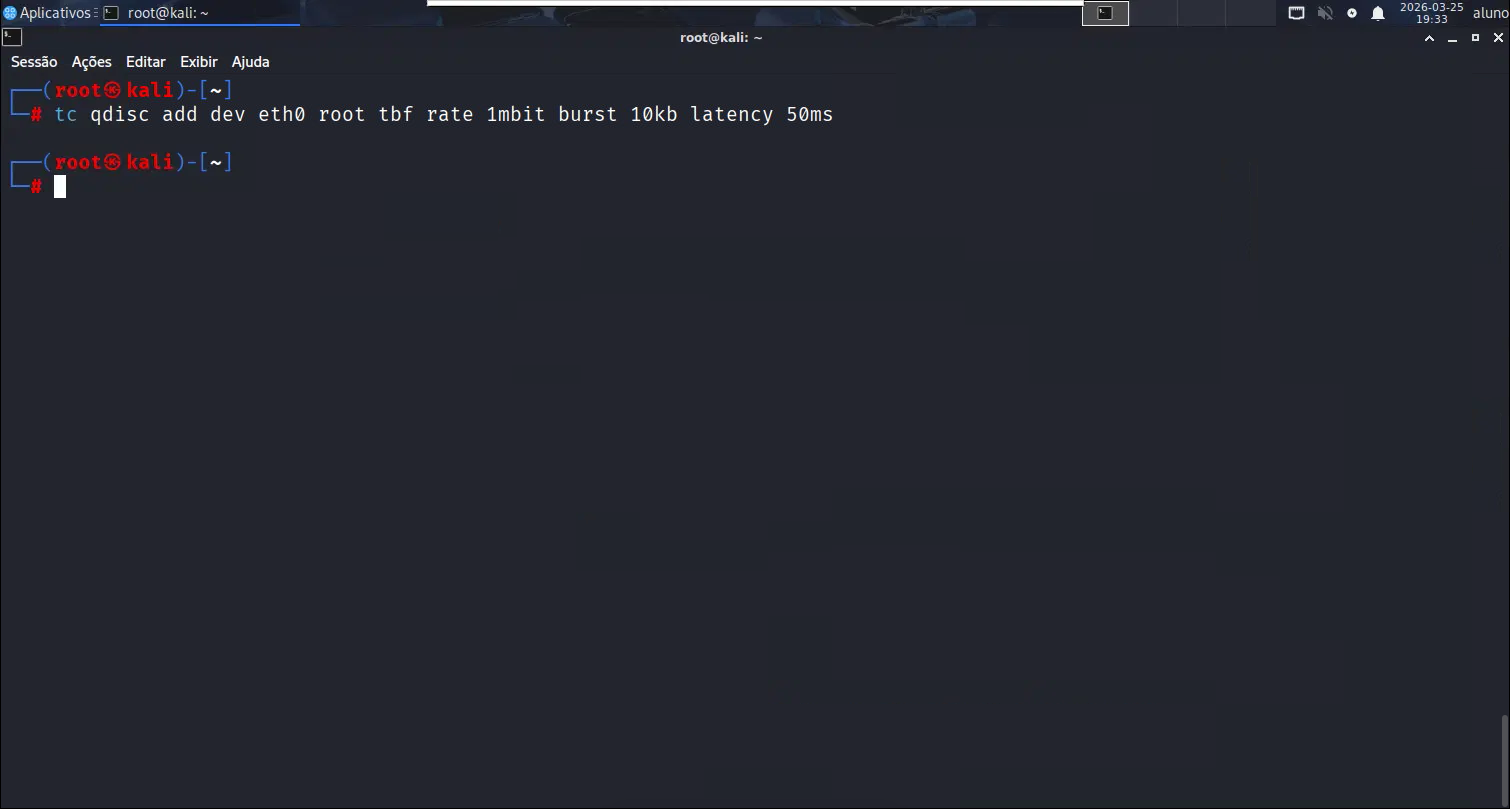
\includegraphics[width=0.99\textwidth]{./fig/fig11.4.png}
\caption{Aplicação de política de QoS com limitação de largura de banda via comando tc}
\label{fig:fig11.4}
\end{figure}

\newpage

\question[Atividade 11.5]{Configurando QoS no Windows Server 2022}

\begin{figure}[H]
\centering
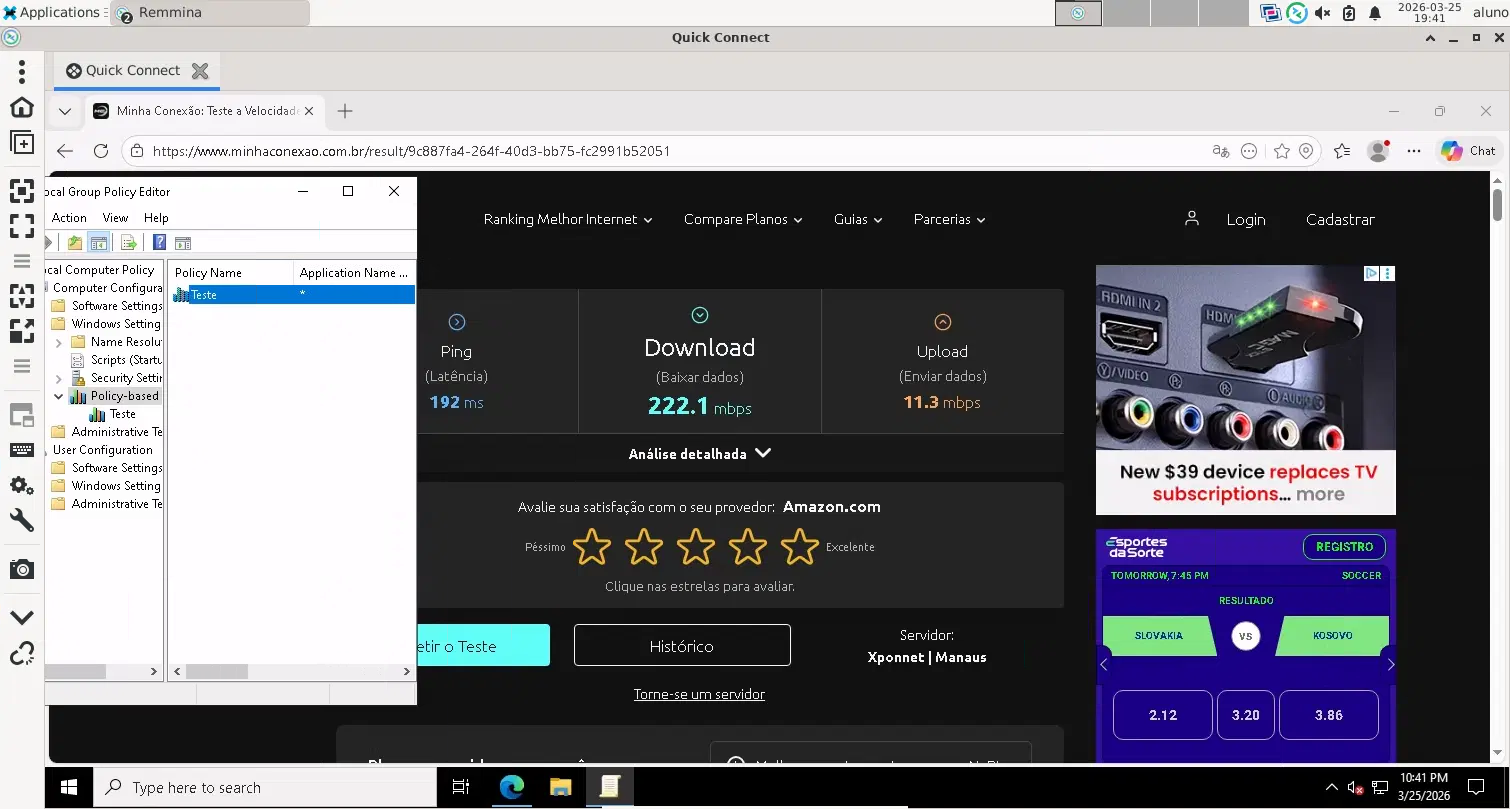
\includegraphics[width=0.99\textwidth]{./fig/fig11.5.png}
\caption{Teste de upload após aplicação da política de QoS com limitação de banda no Windows Server 2022}
\label{fig:fig11.5}
\end{figure}
